\chapter[GROWTH AND DECAY]{\textbf{GROWTH AND DECAY}}
\thispagestyle{empty}
\numberwithin{equation}{chapter}

\section{MALTHUSIAN LAW OF GROWTH}
\par ~~~~~~~~~~The initial value problem $\dfrac{dx}{dt}=kx$ , $x(t_{0})=x_{0}$ where $t$ and $x$ are variables and $k$ is a non zero constant, occurs in many physical theories involving either growth or decay. The constant $k$ can be obtained from the solution of differential equation by using a subsequent measurement of the population at a time \(t_{1}>t_{0}\).The constant $k$ is called the continues growth rate if it is positive, or the continues decay rate if it is negative.

\par ~~~~~~~~There are many quantities in the real world that approximately obey an equation similar to this one. For example population  of animals, radioactivity, temperature of cooling body, amount of substance remaining during a reaction etc. \\
\\ Solving the equation generally,
\begin{center}
	\begin{eqnarray*}
			\frac{dx}{dt}&=kx   \\ 
			and ~~~~~~  
		{\frac{dx}{dt}}.{\frac{dt}{dx}}&=1  \\
		\implies ~~~~~~~~
		\frac{dt}{dx}&=\frac{1}{kx}
	\end{eqnarray*}
\end{center}
$$t=\dfrac{1}{k}logx+c$$
$$x=e^{k(t-c)}$$
~~~~~~~~~~~~~~~~~~~~~~~~~~~~~~~~~~~~~or~~~~~~~~
$x(t)=Ce^{kt}$ \\
Depending on whether k is positive or negative the quantity x grows or decay with respect to t as shown in following graphs

%GRAPH

\begin{center}
	\scalebox{1.00} % Scale down to 70 /% of the original size!
	{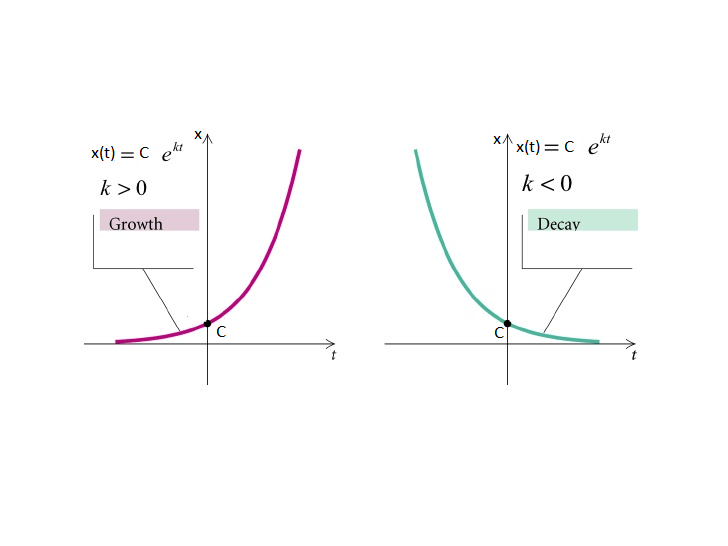
\includegraphics{graph3.png}}
\end{center}

The fundamental differential equation $\frac{dx}{dt}=kx$ with solution $x=ce^{kt}$ is called Malthusian law of growth named after T R Malthus(1766-1834)


\subsection*{Example} 

\par ~~~~~~~~~~Bacteria in a certain culture increase at a rate proportional to the number present. If the number doubles in one hour, how long does it take for the number to triple?\\                
\\
\textit{\Large Solution}

\par ~~~~~~~~~~Let $y$ denote the numbers present at time $t$. Then the function denoted by $y = f(t)$, satisfies the differential equation $ \frac{dy}{dt}=ky $ and the conditions $t = 0$, $y = y_{0}$; $t = 1$, $y = 2y_{0}$. 
\\
\\
Writing the differential equation in linear form, \\
%\begin{align*}
\begin{center}
	\begin{eqnarray*}
		 		\frac{dy}{y}&=kdt \\
		 		\implies ~~~~~~	  logy&=kt+c \\ 
		  		y&=ce^{kt} \\
		 		y(t=0)=y_{0}  \implies     y_{o}&=c \\
 		 		y(t=1)=2y_{0} 	\implies 2y_{0}&=y_{0}e^{k(1)} \\
 		 		\\
 		 		\linebreak
 				\implies~~~~~~~ 	k&=\log2 \\
 				\therefore ~~~~~~	y&=y_{0}e^{t\log2} \\
	\end{eqnarray*}
\end{center} 


Now $y=3y_{0}$ and solving for t yields
\begin{center}
	\begin{eqnarray*}			
 				3y_{o}&=y_{0}e^{t\log2} \\
 				\implies ~~~~  \log3&=t\log2 \\
 	\end{eqnarray*}
\end{center}
               
		

 Hence, the number will be triple in 
$$t=\frac{log3}{log2}=1.5849 hr$$ 


 


\pagebreak

\section{BIOLOGICAL GROWTH-\\VERHULST PEARL MODEL}


\par ~~~~~~~~A fundamental problem in biology is that of growth, whether it is the growth of a cell, an organ, a human, a plant or population.

\par ~~~~~~~~~~~~We already have the fundamental differential equation $\dfrac{dN}{dT}=kN$ and the solution $N=N_{0}e^{kt}$. One obvious drawback of Malthusian law of growth is that if $k>0$ then we have $N\rightarrow \infty$ as $t\rightarrow \infty$, so that as time passes, growth is unlimited. This conflicts with reality, for after a certain period of time, we know that a cell or individual stops growing having attained a maximum size. So we shall now modify those equations to include these biological facts as follows:

\par ~~~~~~~~~~Suppose N denotes the size of a cell and assume that the rate of change of size depends on the size in a more complicated manner than simple proportionality.  \\
\linebreak
~~~~~~~~Thus, let $\frac{dN}{dT}=F(N)$, $N(t=0)=N_{0}$ where $N_{0}$ represents the size at some specified time, t=0, and F is some suitable function but as yet unknown. Since the linear function $F(N)=kN$ is not suitable, we consider a next order of approximation given by a quadratic function $F(N)=aN-bN^{2}$, where we choose constant $b>0$ in order to inhibit the growth of N as demanded by reality.
\\
Thus, \begin{center}
	$\frac{dN}{dT}=aN-bN^{2}$  ~~, 
	~~~~~~~~~~	$N=N_{0}$ for t=0.
\end{center}

This Equation is termed as a logistic equation and the growth governed by it is called logistic growth. The model represented by this equation is referred to as the \textit{Verhulst-Pearl model}.
\\Now
\begin{center}
	~~~~~~~~  ~~~~	$ \dfrac{dN}{dt}=aN-bN^{2} $
\end{center} 

Separating the variables $~~~~~~~~~~\implies$ 
$ ~~~~~~~~~~\dfrac{dN}{aN-bN^{2}}=dt $ \\

Integrating 
\begin{center}
	\begin{eqnarray*}
		\int\dfrac{1}{aN-bN^{2}}dN&=\int dt \\
		\dfrac{1}{a}\int[\dfrac{1}{N}+\dfrac{b}{a-bN}]dN&=t+c \\
		\frac{1}{a}[\log N-\log(a+bN)]&=t+c \\
	\end{eqnarray*}
\end{center}

%\begin{equation*}
$N(t=0)=N_{0}$ ~~~~ $\implies$  ~~~~
$\dfrac{1}{a}[\log N_{0}-\log(a-bN_{0})]=c$
 \begin{center}
	\begin{eqnarray*}
		\therefore ~~~~   
		\dfrac{1}{a}[\log N-\log(a+bN)]&=t+\dfrac{1}{a}[\log N_{0}-\log(a-bN_{0})] \\
		N&=\dfrac{a}{b+e^{-at}[\frac{a}{N_{0}}-b]} \\
		&=\dfrac{\frac{a}{b}}{1+[\frac{\frac{a}{b}}{N_{O}}-1]e^{-at}} \\
	\end{eqnarray*}
\end{center}
\par This is known as the Verhulst formula.If $t\rightarrow \infty$ we get  (since  a>0) $$N_{max}=\lim_{t\rightarrow \infty}N=\frac{a}{b}$$      which shows that there is a limit to the growth of N as desired by the biological facts and tends to indicate the correctness of our mathematical model.

Suppose that at times $t=1$ and $t=2$, the values of N are $N_{1}$ and $N_{2}$ respectively, then
\begin{center}
	\begin{eqnarray*}
			N_{1}&=\frac{\frac{a}{b}}{1+[\frac{\frac{a}{b}}{N_{0}}-1]e^{-a}}  \\
			and~~~~ 
			N_{2}&=\frac{\frac{a}{b}}{1+[\frac{\frac{a}{b}}{N_{0}}-1]e^{-2a}}
	\end{eqnarray*}
\end{center}
 
\begin{center}
	\begin{eqnarray*}
		Hence~~~~~~
			\dfrac{b}{a}(1-e^{-a})&=\dfrac{1}{N_{1}}-\frac{e^{-a}}{N_{0}} \\
			and~~~~ 
			\dfrac{b}{a}(1-e^{-2a})&=\dfrac{1}{N_{2}}-\frac{e^{-2a}}{N_{0}} 
	\end{eqnarray*}
\end{center}

\begin{center}
	\begin{eqnarray*}
			\implies ~~~
			1+e^{-a}&=\frac{\frac{1}{N_{2}}-\frac{e^{-2a}}{N_{0}}}{\frac{1}{N_{1}}-\frac{e^{-a}}{N_{0}}} \\
			\\~~
			e^{-a}&=\frac{N_{0}(N_{2}-N_{1})}{N_{2}(N_{1}-N_{0})} \\
	\end{eqnarray*}
\end{center}

$$\frac{b}{a}=\frac{N_{1}^{2}-N_{0}N_{2}}{N_{1}(N_{0}N_{1}-2N_{0}N_{2}+N_{1}N_{2}})$$ 
	\\
Hence the limiting value of N is
$$ N_{max}=\lim_{t\rightarrow\infty}N=\frac{N_{1}(N_{0}N_{1}-2N_{0}N_{2}+N_{1}N_{2})}{N_{1}^{2}-N_{0}N_{2}} $$
\linebreak
The graph of the problem  has the general appearance in the figure.

%GRAPH

\begin{center}
	\scalebox{1.20}
	{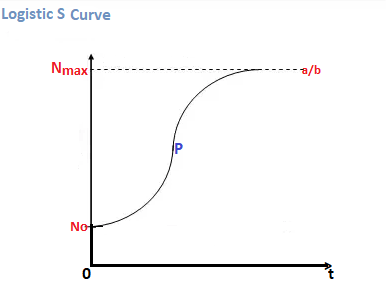
\includegraphics{graph4.png}} %include the image - image is in the working folder
\end{center}


\par ~~~~~~~~~~~~This graph reveals that as t increases from 0, N increases from $N_{0}$ and gets closer to $N_{max}$. The curve has an increasing slope from t=0 to a time corresponding to the point P, and thereafter has a decreasing slope. Thus point P is a point of inflection.
\par ~~~~~~~~~~The S shaped curve in the figure is called the \textit{logistic curve} and has proved to be of great accuracy in predicting the growth patterns in a limited space.

\section*{Example}  
\par ~~~~~~~~~~The mean size of a cell at various stages is shown in Table. Use the data to predict the mean size of adult cell at full growth.  \\
\\    
\newpage  
Mean size of a human cell at Various stages
\\ 
\begin{center}
	\begin{tabular}{|c|c|}
		\hline
		Stage & Size \\
		\hline
		Birth & 19.4 \\
		\hline
		1 & 31.3 \\
		\hline
		2 & 34.5 \\
		\hline
		3 & 37.2 \\
		\hline
		4 & 40.3 \\
		\hline
		5 & 43.9 \\
		\hline
		6 & 48.1 \\
		\hline
		7 & 52.5 \\
		\hline
		8 & 56.8 \\
		\hline
	\end{tabular}
\end{center}                   



~~~~~~~~~~To cover the full set of data given in the table, let t=0,1,2 correspond to the size at birth of cell, 4 and 8 stages, respectively. Thus, we have
$N_{0}=19.4, N_{1}=40.3, N_{2}=56.8$ .
\par  Substituting these values  we get  \\                              $$N_{max}= 66.9$$ which is the required mean size(growth) of a human cell.


